\section[Communications strategies]{Telling people about your work}
\label{sec:communications_strategies}

%---------------------------------------------------------------
% 1. Why do we communicate
%---------------------------------------------------------------

\begin{frame}{Why do we communicate?}

% left empty for student input

\end{frame}

%---------------------------------------------------------------
% 2. Effective communications 
%---------------------------------------------------------------
\begin{frame}{Effective communications make a difference}

\vspace{-0.75cm}
\begin{columns}

    \begin{column}{0.3\textwidth}
        \begin{block}{They make you aware}
        \centering
            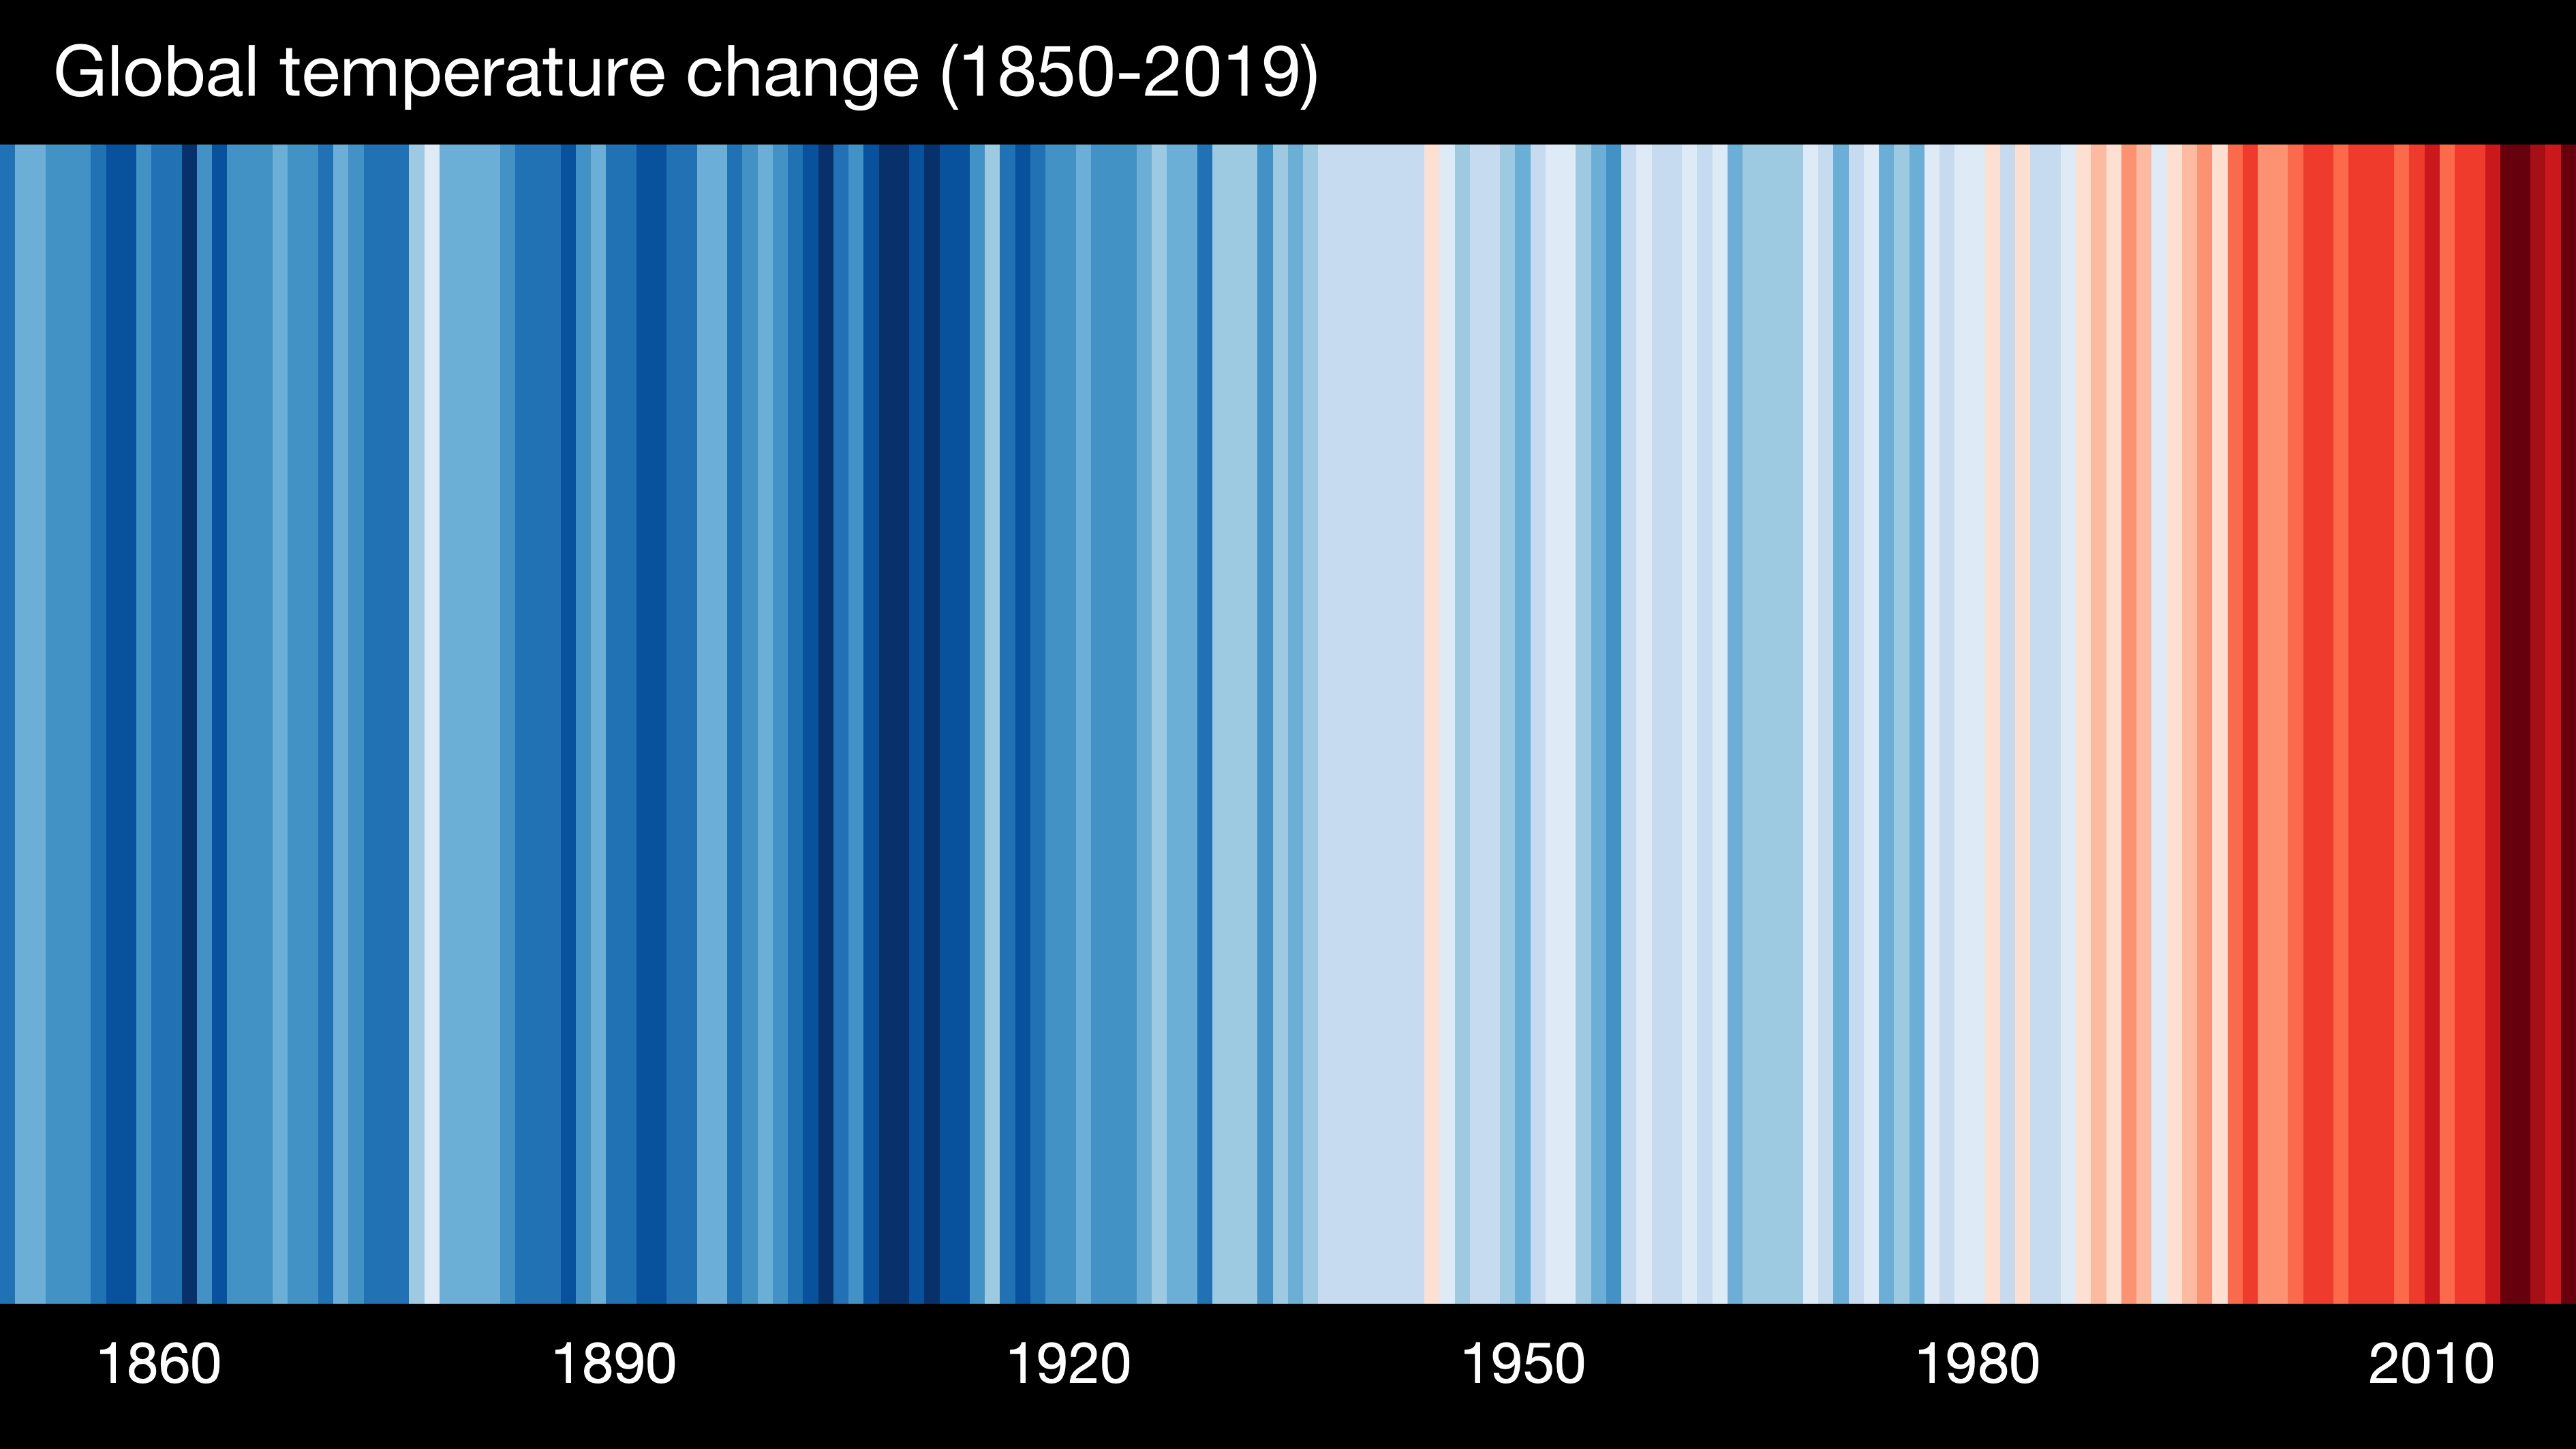
\includegraphics[width=\textwidth]{images/_stripes_GLOBE---1850-2019-MO-withlabels.png}
            \givecredit{\textlink{https://showyourstripes.info/}{Annual average temperatures for the globe}. Image by Ed Hawkins (University of Reading). Used under CC BY 4.0 license.}
        \end{block}
    \end{column}
    
    \begin{column}{0.3\textwidth}
        \begin{block}{They make you care}
        \centering
            
\includegraphics[width=\textwidth]{images/mika-baumeister-9fJidQI2o-s-unsplash.jpg}
            \givecredit{Photo by \textlink{https://unsplash.com/@mbaumi}{Mika Baumeister} on \textlink{https://unsplash.com}{Unsplash}}
        \end{block}
    \end{column}

    \begin{column}{0.3\textwidth}
        \begin{block}{They make you act}
        \centering
            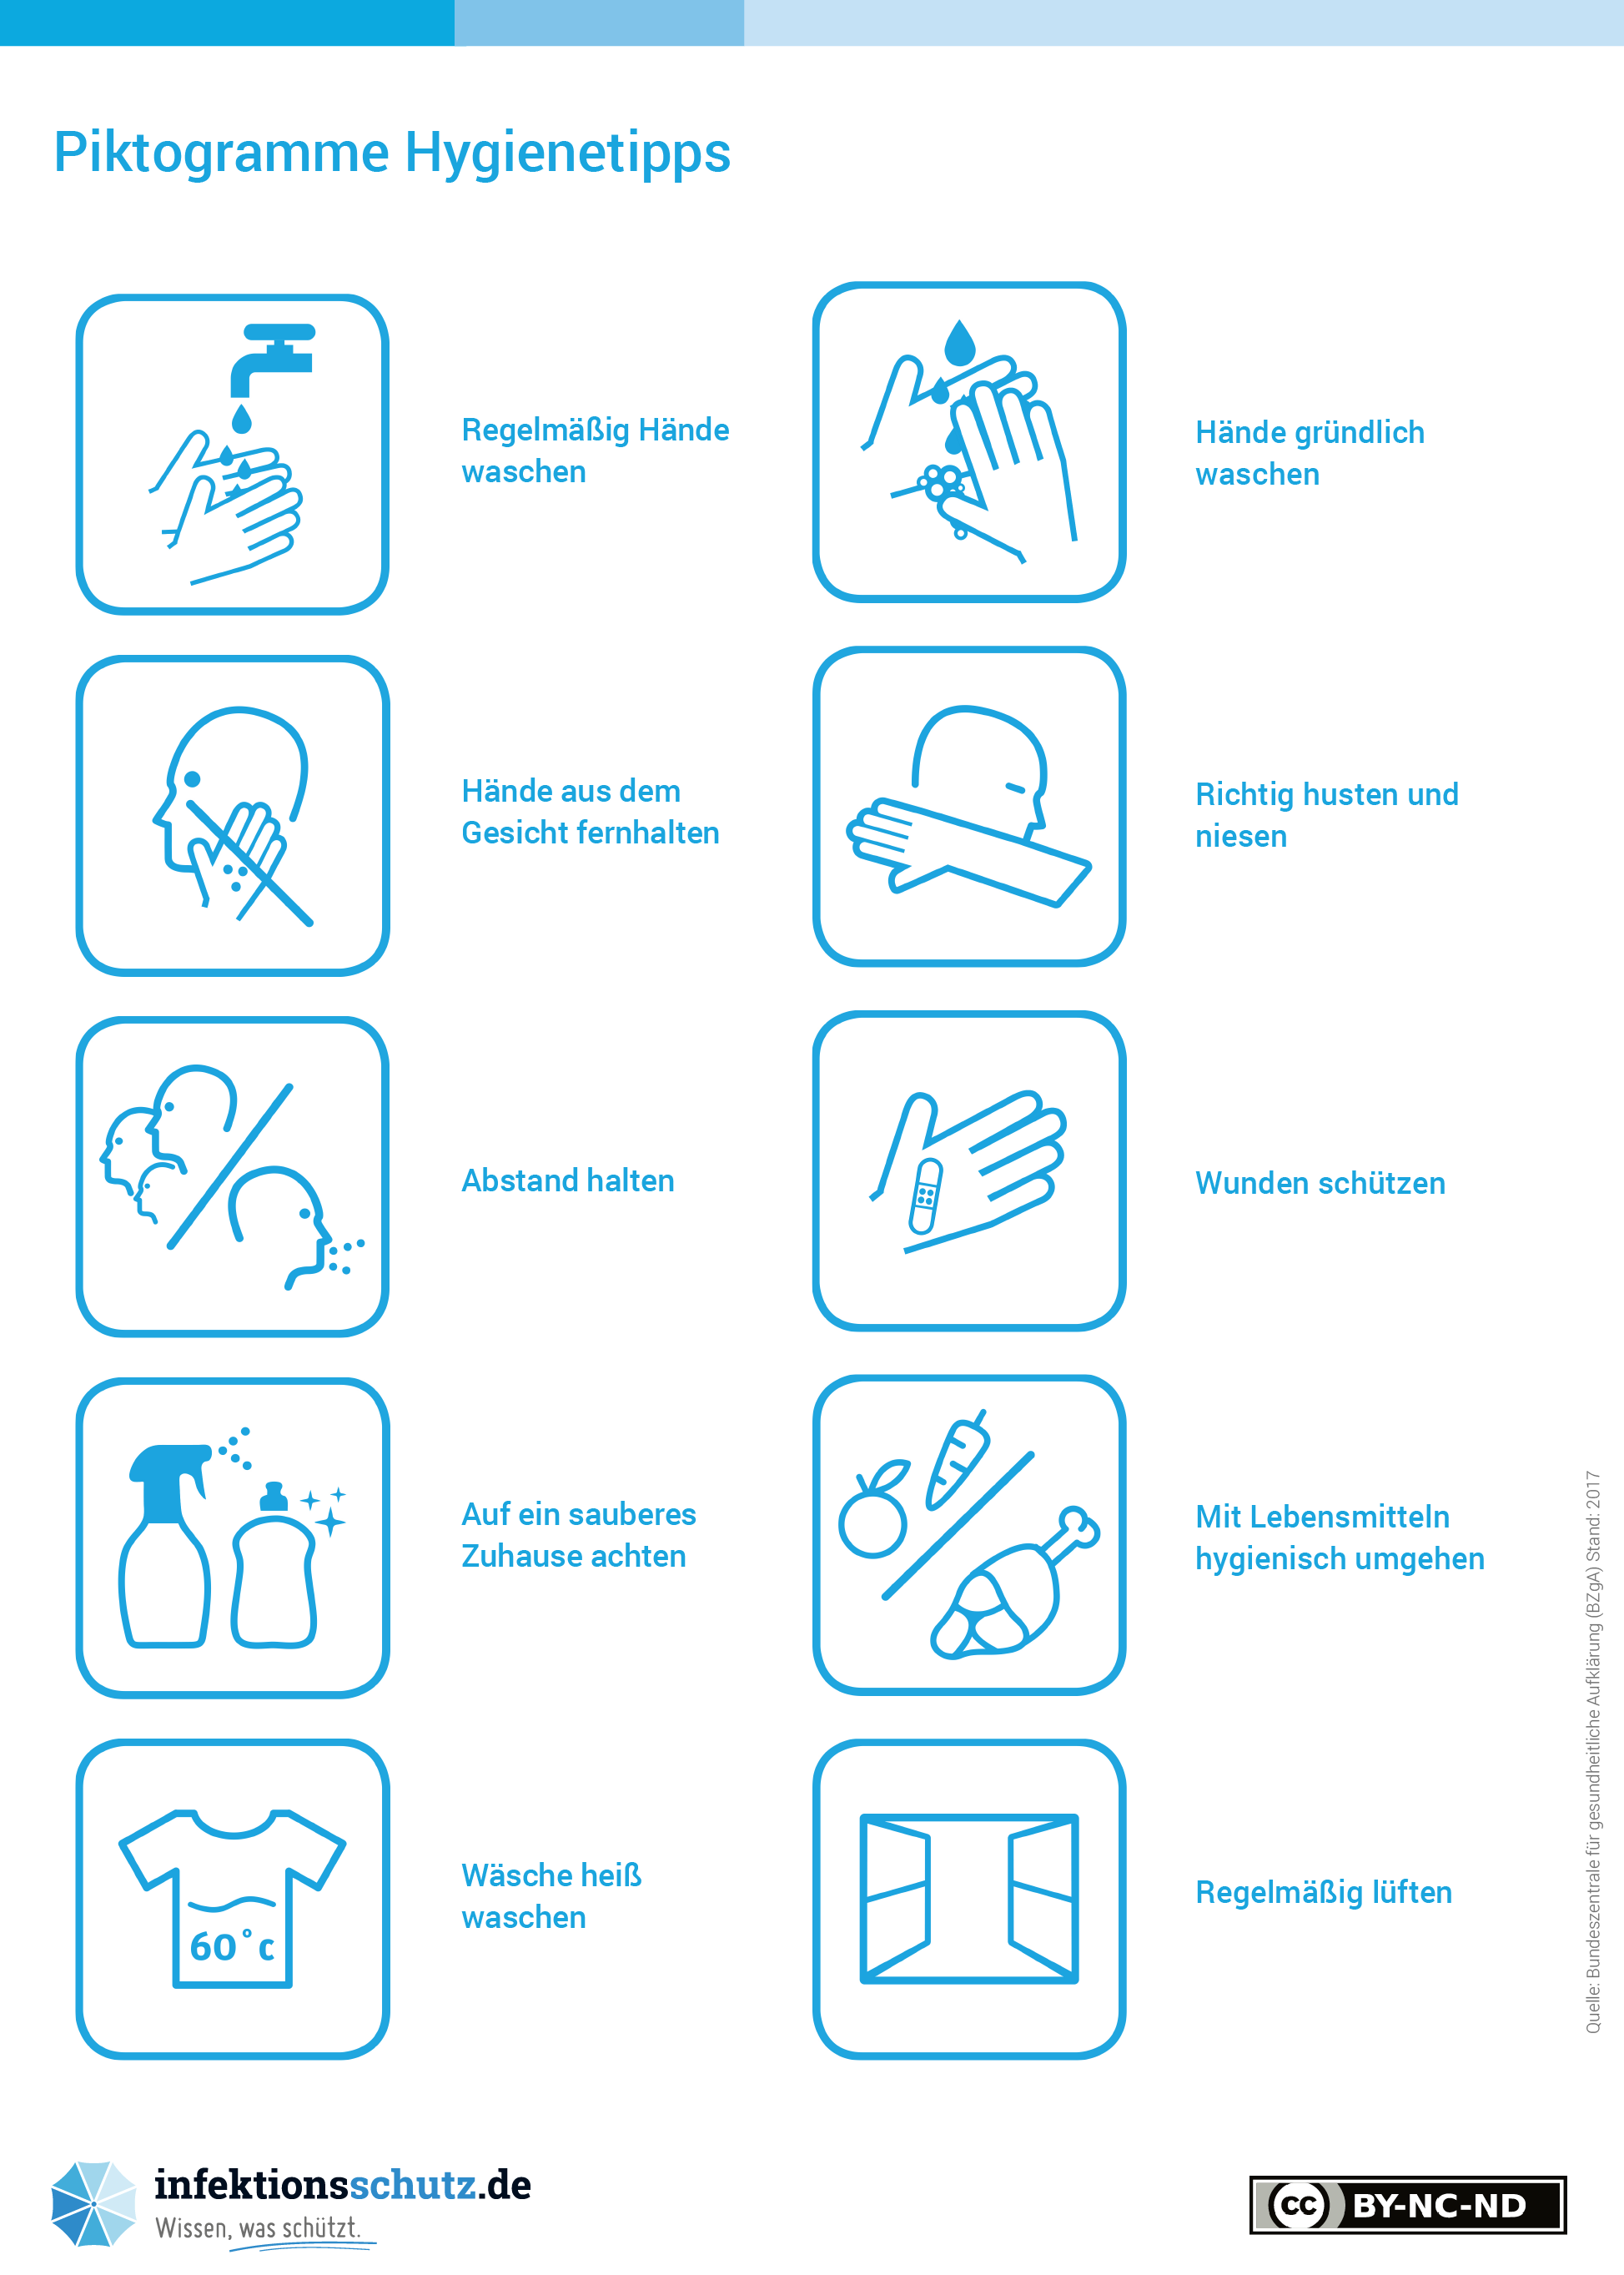
\includegraphics[width=\textwidth]{images/Piktogramme_Hygienetipps_300dpi.png}
            \givecredit{\textlink{https://www.infektionsschutz.de/mediathek/infografiken.html}{German Federal Centre for Health Education (BZgA)}}
        \end{block}

    \end{column}

\end{columns}

\end{frame}

%---------------------------------------------------------------
% 3. Media
%---------------------------------------------------------------

\begin{frame}{Channel - Audience - Message}

\vspace{-0.75cm}
\begin{columns}
    \begin{column}{0.3\textwidth}
        \begin{block}{Apps \& mobile devices}
            \centering
            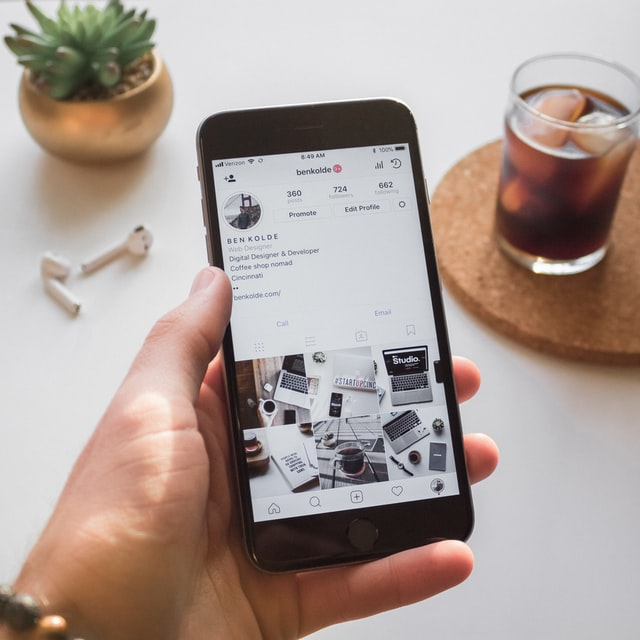
\includegraphics[width=\textwidth]{images/ben-kolde-_zqJaEyo6I4-unsplash.jpg}
            \givecredit{Photo by \textlink{https://unsplash.com/@benkolde}{Ben Kolde} on \textlink{https://unsplash.com}{Unsplash}}
            % some text about the message
            {\small
            \textbf{Audience:} Almost anyone\\
            \textbf{Message:} Call to action. %
            }
        \end{block}
    \end{column}
    
    \begin{column}{0.3\textwidth}
        \begin{block}{Conferences \& Webinars}
        \centering
            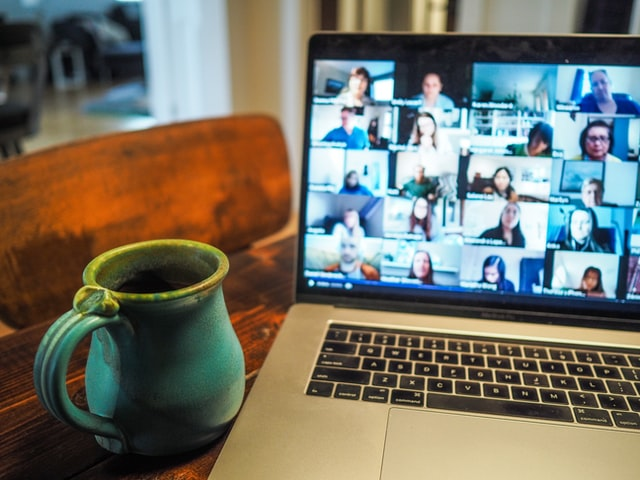
\includegraphics[width=\textwidth]{images/chris-montgomery-smgTvepind4-unsplash.jpg}
            \givecredit{Photo by \textlink{https://unsplash.com/@cwmonty}{Chris Montgomery} on \textlink{https://unsplash.com}{Unsplash}}
            % some text about the message
            {\small
            \textbf{Audience:} Already interested\\
            \textbf{Message:} Insight \& understanding. %
            }
        \end{block}
    \end{column}
    
    \begin{column}{0.3\textwidth}
        \begin{block}{Print*}
        \centering
            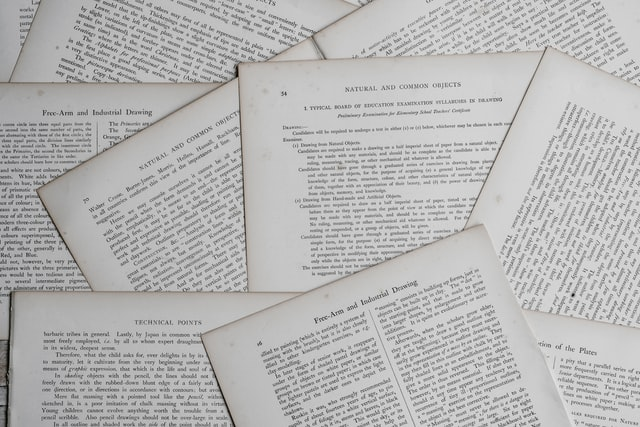
\includegraphics[width=\textwidth]{images/annie-spratt-5cFwQ-WMcJU-unsplash.jpg}
            \givecredit{Photo by \textlink{https://unsplash.com/@anniespratt}{Annie Spratt} on \textlink{https://unsplash.com}{Unsplash}}
            % some text about the message
            {\small
            \textbf{Audience:} \emph{Really} interested\\
            \textbf{Message:} Actionable information. %
            }
        \end{block}
    \end{column}
    
\end{columns}

\end{frame}

%---------------------------------------------------------------
% 4. New Media
%---------------------------------------------------------------

\begin{frame}{Are there better ways to reach your audience?}
\centering
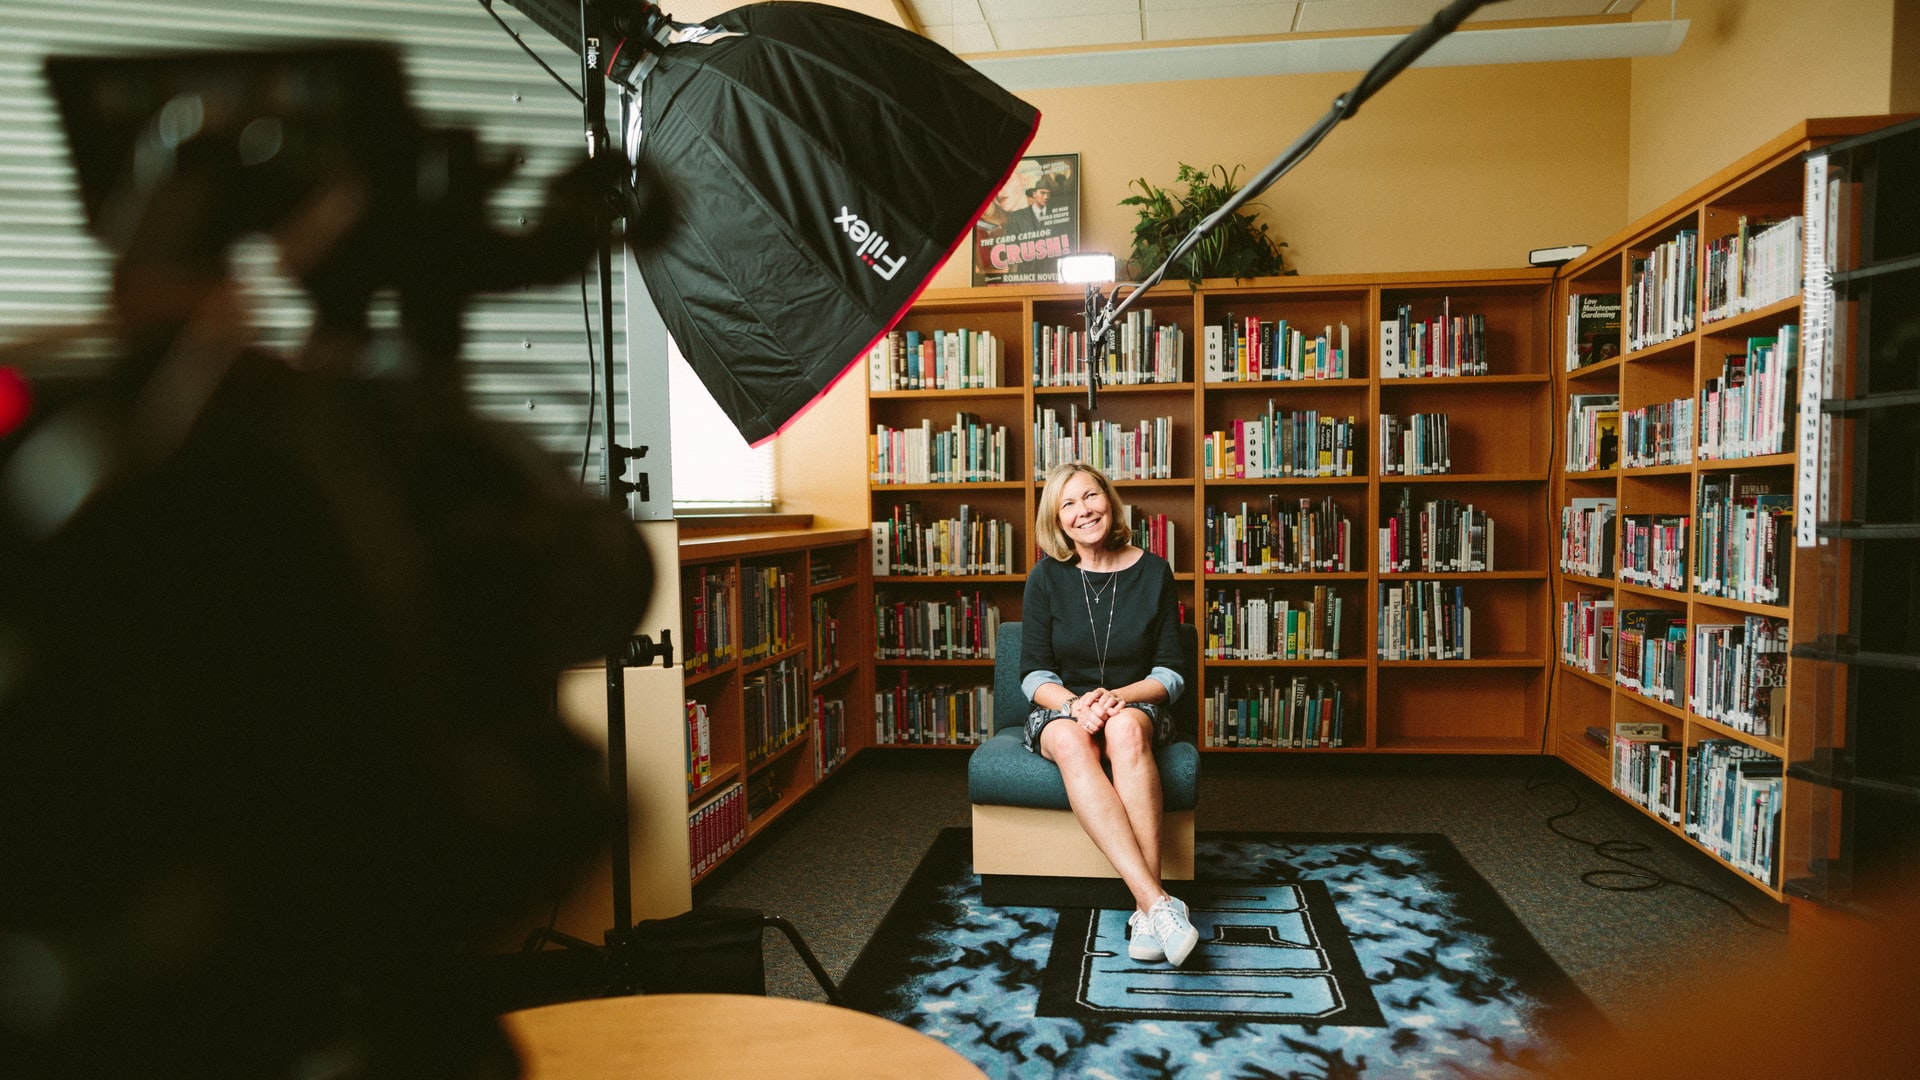
\includegraphics[height=0.7\textheight]{images/sam-mcghee-4siwRamtFAk-unsplash.jpg}

\givecredit{Photo by \textlink{https://unsplash.com/@sammcghee}{Sam McGhee} on \textlink{https://unsplash.com}{Unsplash}}
\end{frame}

%---------------------------------------------------------------
% 5. Tell your story
%---------------------------------------------------------------

\begin{frame}{And now, you tell your story}
\centering
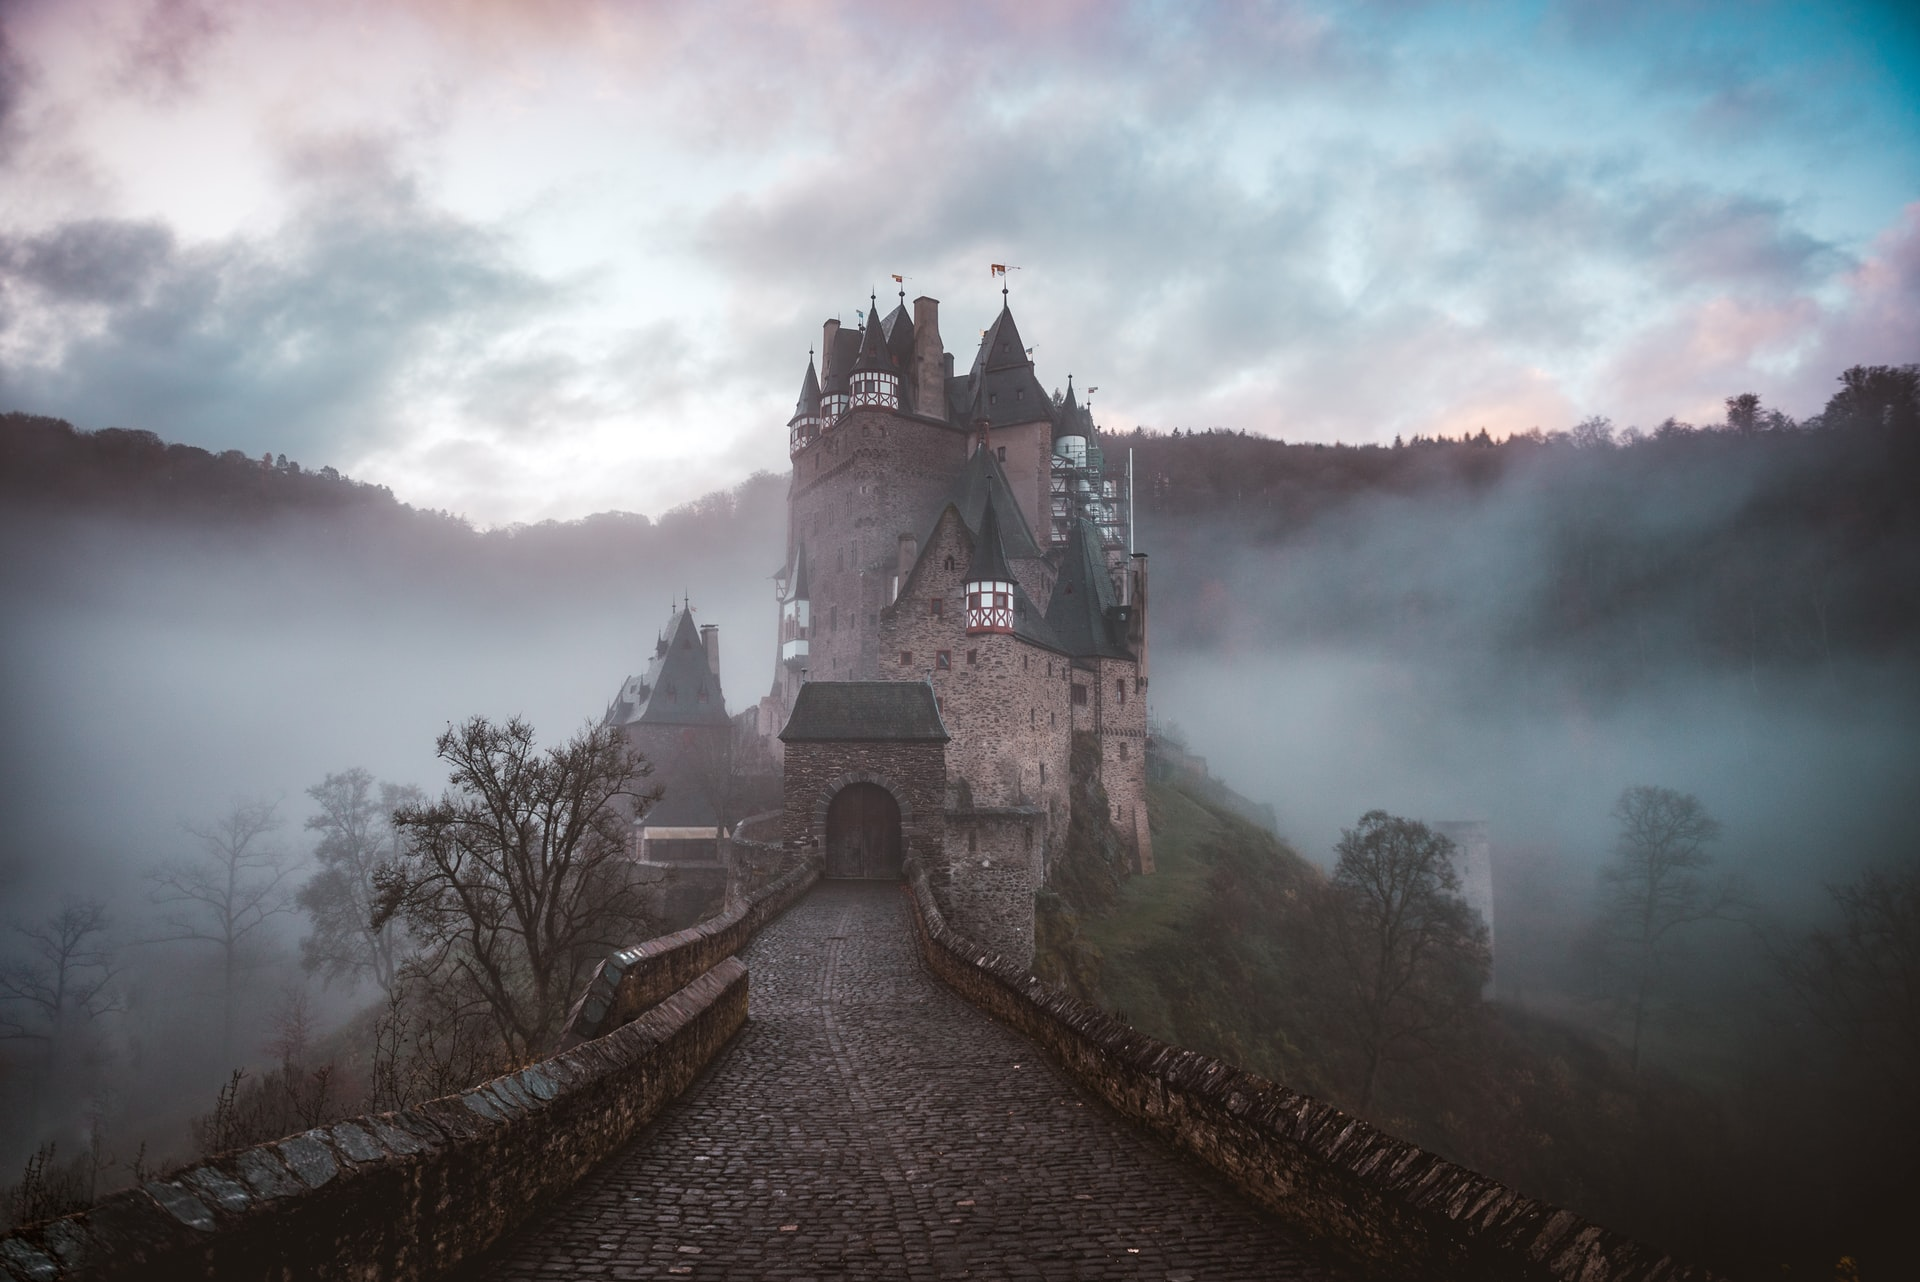
\includegraphics[height=0.7\textheight]{images/cederic-vandenberghe-21DP3hytVHw-unsplash.jpg}

\givecredit{Photo by \textlink{https://unsplash.com/@cedericvandenberghe}{Cederic Vandenberghe} on \textlink{https://unsplash.com}{Unsplash}}
\end{frame}

%---------------------------------------------------------------
% 6. How we make effective communications
%---------------------------------------------------------------
\begin{frame}{Designing a communications strategy}

\begin{columns}

    \begin{column}{0.45\textwidth}
        \begin{minipage}[t][.7\textheight]{\textwidth}
        
        Figure out why you are communicating:
        \begin{itemize}
            \item Who's the audience?
            \item What do you want them to do?
            \item How does your communication help?
        \end{itemize}
        \vfill
        Work out how to achieve that goal:
        \begin{itemize}
            \item To make people aware: inform
            \item To make people care: persuade
            \item To make people act: push or provoke
        \end{itemize}
        \vfill
        Choose your media
        \vfill
        Tell your story
        \end{minipage}
    \end{column}

    \begin{column}{0.45\textwidth}

    \end{column}

\end{columns}


%---------------------------------------------------------------
% 7. Is this a good example?
%---------------------------------------------------------------

\begin{frame}[plain]
    % blog post + linkedin + article + uni press release
    
    \centering
    % image illustrating a communications campaign

\usetikzlibrary{positioning}
\usetikzlibrary{overlay-beamer-styles}

\begin{tikzpicture}[remember picture, overlay]

    % NREL press release
    \node[anchor=south west, xshift=0.25cm](NREL) at (current page.south west) {
        
\includegraphics[height=150pt]{images/eaau2027_NREL_pressrelease.png}
    };

    % DTU press release
    \node[anchor=north west](DTU) at (current page.north west) {
        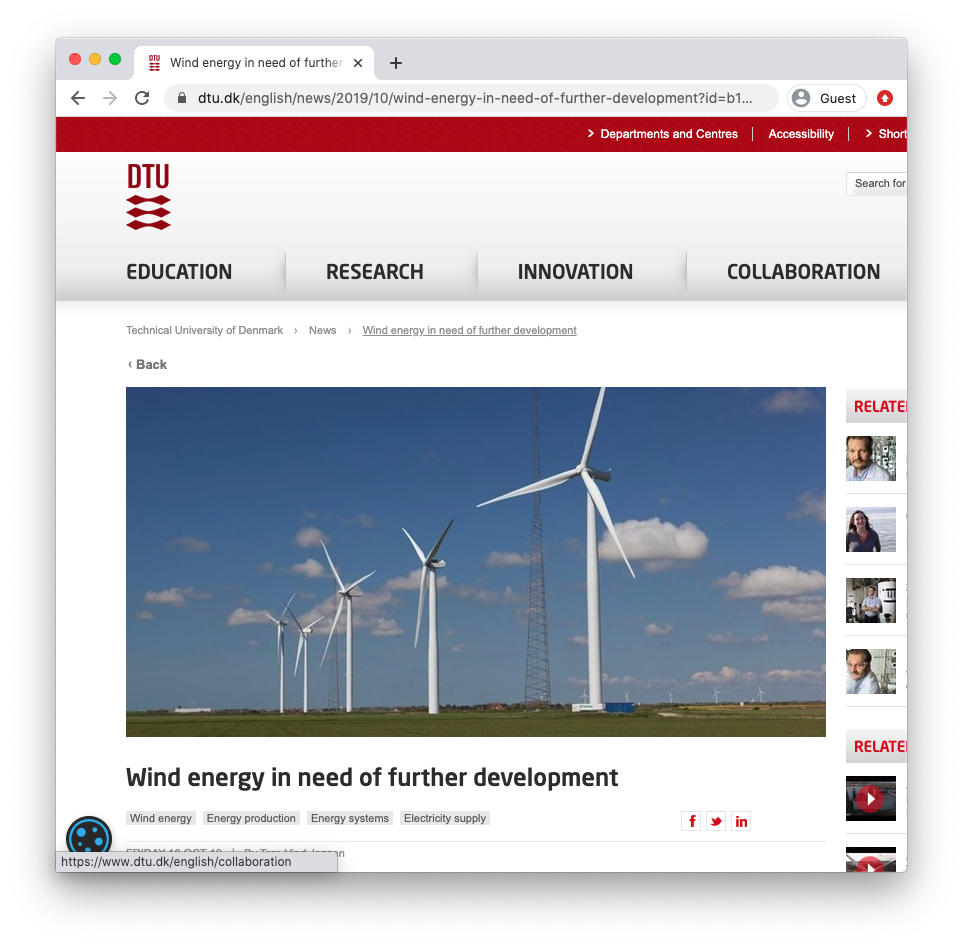
\includegraphics[height=150pt]{images/eaau2027_DTU_pressrelease.png}
    };
    
    % Conference picture
    \node[anchor=north east, xshift=-0.25cm](Conf) at (current page.east) {
        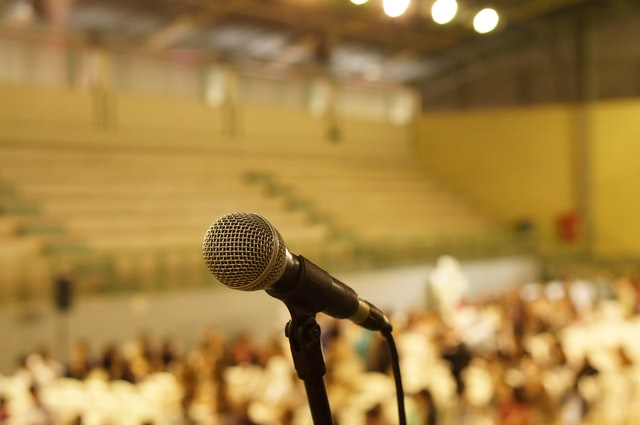
\includegraphics[height=100pt]{images/joao-cruz-IkEpl3JkVqU-unsplash.jpg}
    };
    
    % Article from wind power monthly
    \node[anchor=north east](WPM) at (current page.north east) {
        
\includegraphics[height=150pt]{images/eaau2027_WPM.png}
    };
    
    % linkedin logo
    \node[anchor=east, yshift=-0.75cm](L) at (current page.east) {
        \colorbox{white}{
\includegraphics[height=25pt]{images/LI-Logo.png}}
    };
    
    
    % paper
    \node[line width=1mm](Sci) at (current page.center) {
        \frame{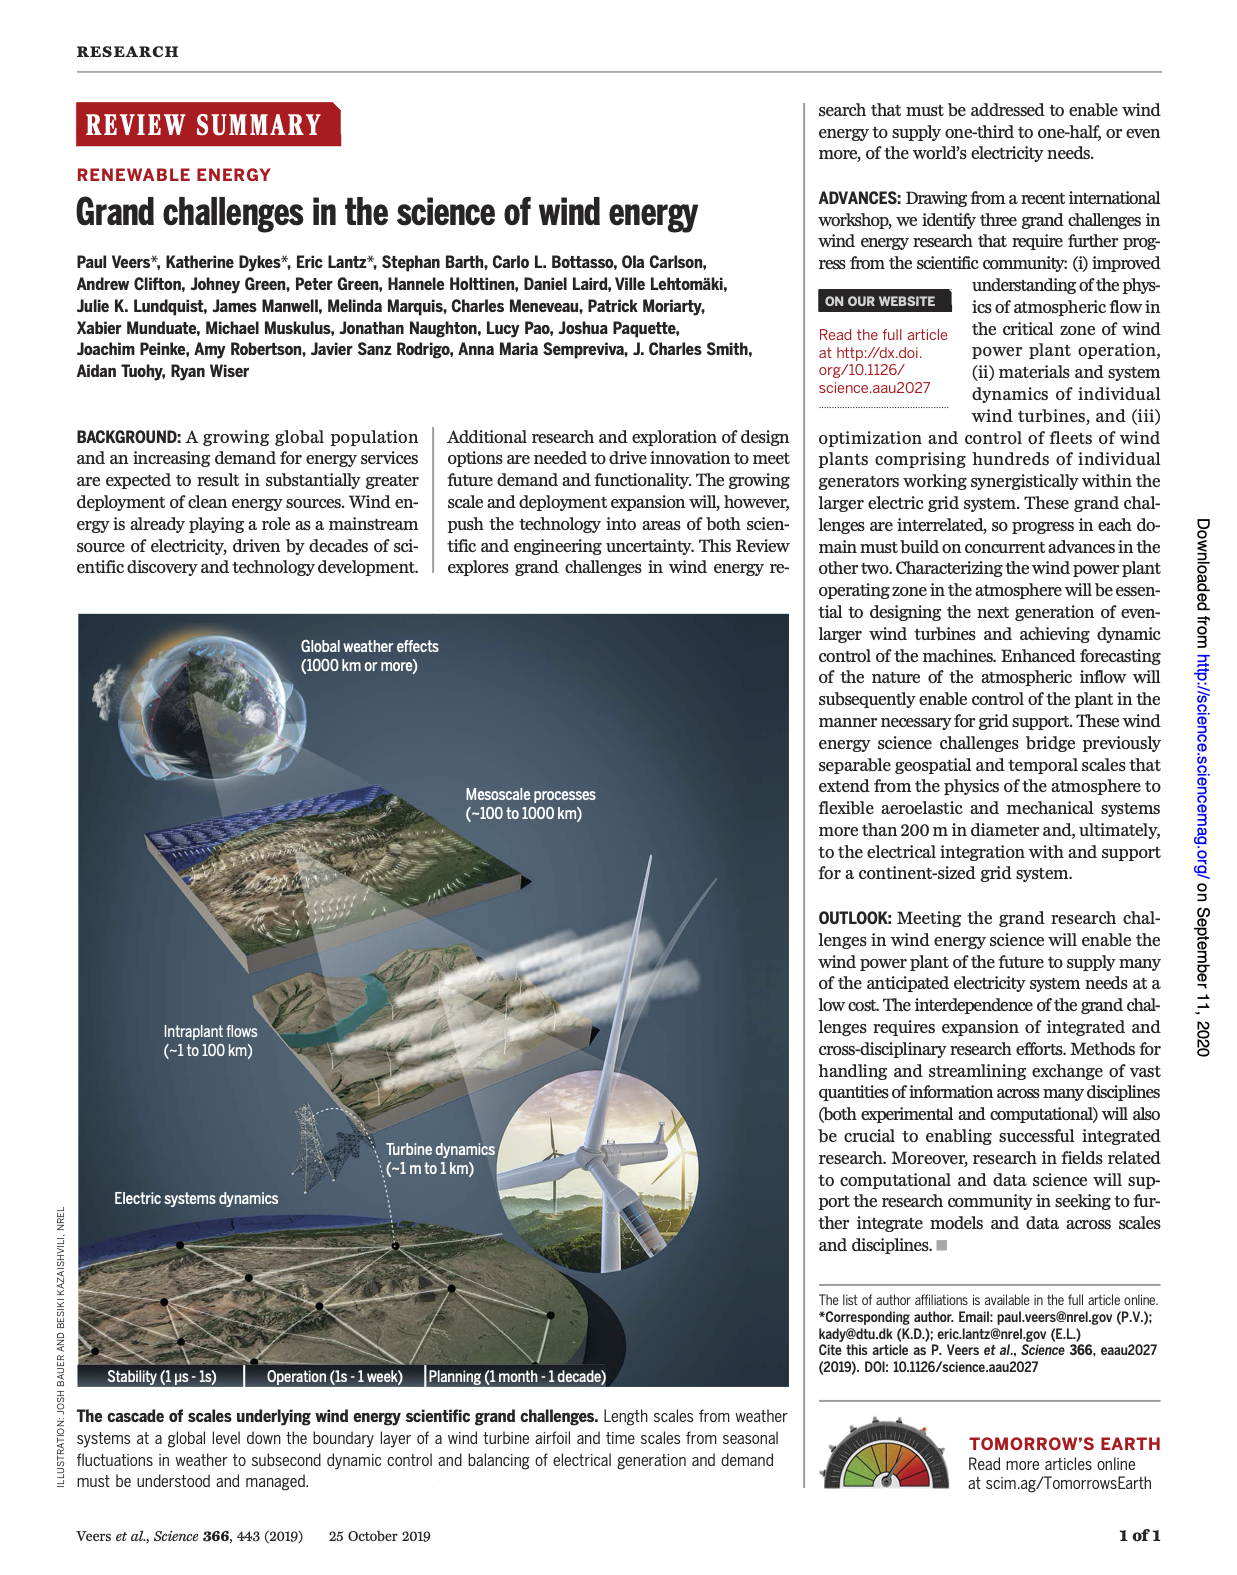
\includegraphics[height=0.9\paperheight]{images/eaau2027_front.png}}
    };    

\end{tikzpicture}

    
    \end{frame}

\end{frame}